
Une brève introduction à la technologie Bluetooth est présentée dans la \cref{sec-stateoftheart_ble}. La présente section a pour but d'expliquer plus en détail cette technologie. Celle-ci ayant été activement utilisée dans ce projet, il est important de comprendre ses bases.

Le Bluetooth opère dans la plage de fréquence ISM (\textit{Industrial, Scientific et Medical}) de 2.4 à 2.4835 GHz. L'on peut visualiser les répartitions de cette bande à l'aide de la \cref{fig-ble_channels_vs_802} en examinant les 40 canaux du BLE. Parmi ces canaux, 37 sont réservés à la communication de données. Les trois autres sont réservés à l'émission d'\textit{advertisements} (voir \cref{sec-protocol_ble_adv} pour plus d'informations) pour établir des connexions ou pour diffuser des informations. L'on remarque également que le WiFi (nommé 802.11 sur la \cref{fig-ble_channels_vs_802}) se trouve sur la même fréquence. Les différents canaux WiFi (au nombre de 13 en Europe) se superposent sur cette bande, ce qui implique qu'il puissent perturber les communications sur cette bande de fréquence. Pour pallier à ces interférences, le Bluetooth effectue du \textit{frequency-hopping spread spectrum}\footnote{\url{https://en.wikipedia.org/wiki/Frequency-hopping_spread_spectrum}}, ce qui signifie qu'il change régulièrement de canal dans un pattern pseudo aléatoire connu des deux dispositifs. \\

\begin{figure}[ht!]
    \centering
    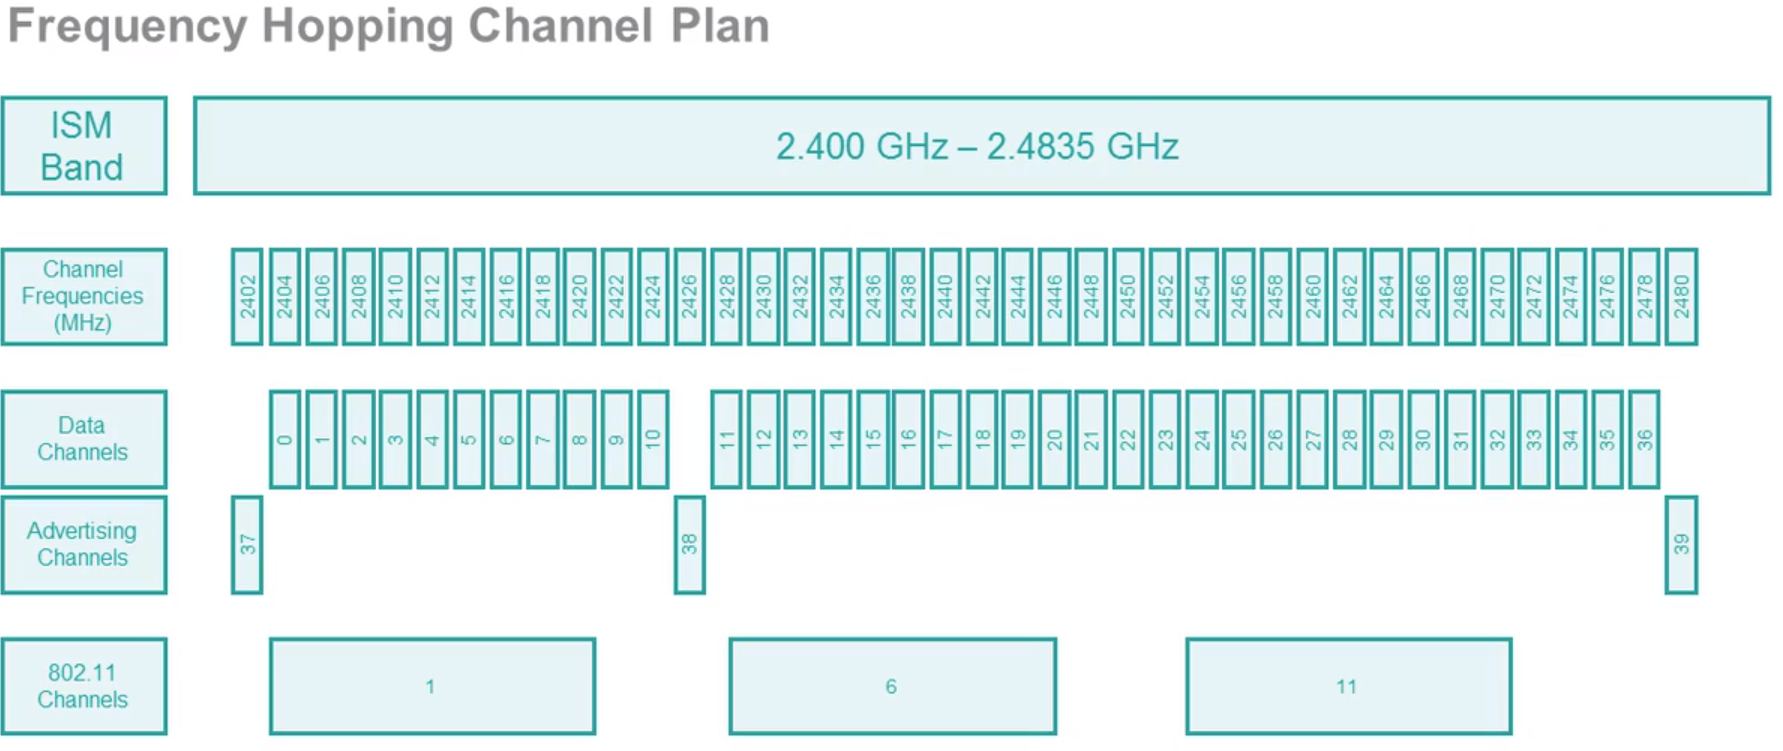
\includegraphics[width=1.0\textwidth]{Figures/Protocols/Bluetooth/ble_channels_vs_802_11.PNG}
    \caption{Bande ISM utilisée par le Bluetooth Low Energy}
    \label{fig-ble_channels_vs_802}
\end{figure}

Le Bluetooth Low Energy utilise la modulation Gaussian Frequency Shift Keying \footnote{\url{https://en.wikipedia.org/wiki/Frequency-shift_keying\#Gaussian_frequency-shift_keying}} (GFSK).  La différence entre le Bluetooth Low Energy et le Bluetooth Classic réside dans l'index de la modulation qui s'élève à 0.35 pour le \textit{Classic} et 0.5 pour le Low Energy \cite{BluetootModulation:online}.

\subsection{Interopérabilité entre les dispositifs}

La \cref{sec-stateoftheart_ble} explore la différence entre le Bluetooth et le Bluetooth Low Energy, mais il faut savoir que certains problèmes d'incompatibilité persistent entre les deux technologies. En réalité, il existe deux mondes. Le premier est celui du Bluetooth \textit{standard} ou \textit{classic}, les dispositifs communiquant dans ce monde sont labellisés \textit{Bluetooth}. Le deuxième monde est celui des dispositifs communiquant en Low Energy, ces dispositifs ont le label \textit{Bluetooth Smart}. Ces derniers ne peuvent pas communiquer avec les premiers et vice-versa. La communication entre les deux mondes est réservée aux dispositifs de type \textit{Bluetooth Smart Ready}. De moins en moins de dispositifs ne sont labellisés que Bluetooth, mais il existe encore de vieux appareils qui ne sont pas \textit{Smart Ready}. De nos jours, tous les smartphones sont \textit{Smart Ready}. La communication entre ces deux mondes est visible sur la \cref{fig-bluetooth_interoperabilty}.



\begin{figure}[ht!]
    \centering
    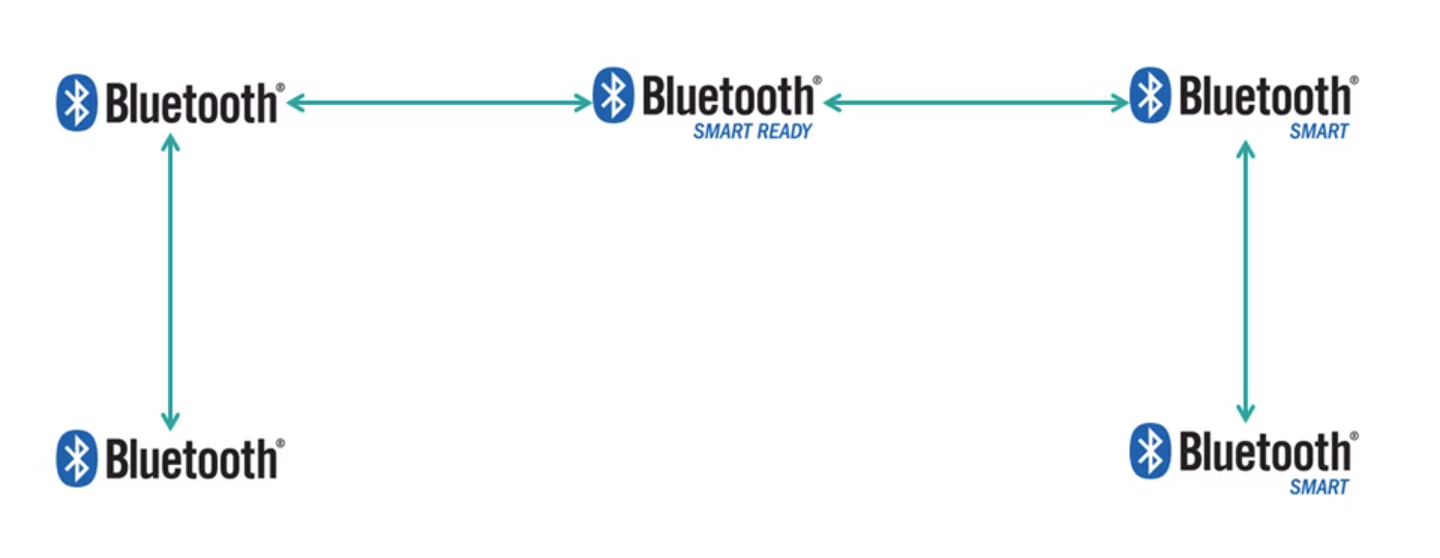
\includegraphics[width=0.7\textwidth]{Figures/Protocols/Bluetooth/bluetooth_interoperabilty.PNG}
    \caption{Interopérabilité entre les dispositifs Bluetooth}
    \label{fig-bluetooth_interoperabilty}
\end{figure}


\subsection{Rôles}
\label{sec-protocol_ble_roles}


En Bluetooth Low Energy, quatre terminologies décrivent les objets souhaitant établir une connexion Bluetooth et échanger des informations une fois connectés. La \cref{fig-central_vs_peripheral} illustre ces quatre terminologies. En premier lieu, il y a les objets en eux même, soit sur l'illustration un capteur de fréquence cardiaque. Ensuite, un smartphone ou PC qui souhaite récupérer les données ce cet objet. Un dispositif qui souhaite engager la connexion porte le nom de \textbf{centrale}. Le dispositif acceptant la connexion est quant à lui nommé \textbf{périphérique}. Une fois la connexion établie, il est possible d'échanger des données. Là, les noms ne sont plus les mêmes, car c'est maintenant le rôle des services Bluetooth de fournir les données (cf. \cref{sec-protocols_BLE_services}). La centrale est nommée \textbf{client}, tandis que le périphérique est le \textbf{serveur}. Les dispositifs Bluetooth sont tous identifiés à l'aide d'une adresse MAC\footnote{\url{https://en.wikipedia.org/wiki/MAC_address}} unique sur 48 bits envoyée dans tous les paquets, y compris lorsqu'une connexion doit être établie. \\

\begin{figure}[ht!]
    \centering
    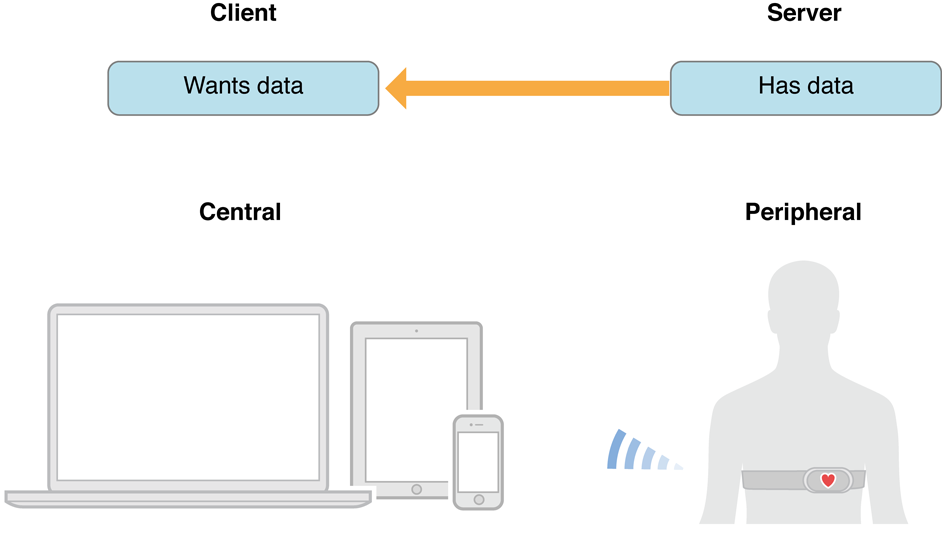
\includegraphics[width=0.7\textwidth]{Figures/Protocols/Bluetooth/central_vs_peripheral.png}
    \caption{Terminologies des connexions et des échanges de données en Bluetooth Low Energy}
    \label{fig-central_vs_peripheral}
\end{figure}

Parfois les termes «central» et «périphérique» sont remplacés par les notions de \textbf{maitre} et \textbf{esclave}, car comme dans beaucoup de protocoles, le maitre initialise la connexion (ou communication) avec l'esclave.

\subsection{\textit{Advertisements}}
\label{sec-protocol_ble_adv}

Un périphérique Bluetooth Low Energy doit s'annoncer lorsqu'il est prêt pour être connecté ou simplement quand il souhaite informer ses voisins de sa présence. Lors de la présentation des canaux Bluetooth (cf. \cref{fig-ble_channels_vs_802}), on peut constater la présence de trois canaux réservés aux \textit{advertisements}. Ceux-ci ont deux rôles. Le premier est d'annoncer à une centrale que le périphérique est disponible ou non pour une connexion BLE. Le second consiste à diffuser à toutes les centrales et périphériques aux alentours un paquet de données personnalisable par l'utilisateur. Cette dernière catégorie contient le concept de \textit{beacons}, lequel est abordé dans la \cref{sec-protocols_BLE_beacons} de ce document. Le choix du canal d'\textit{advertisements} est aléatoire (parmi les trois présentés) pour chaque nouveau paquet envoyé. \\

\begin{figure}[ht!]
    \centering
    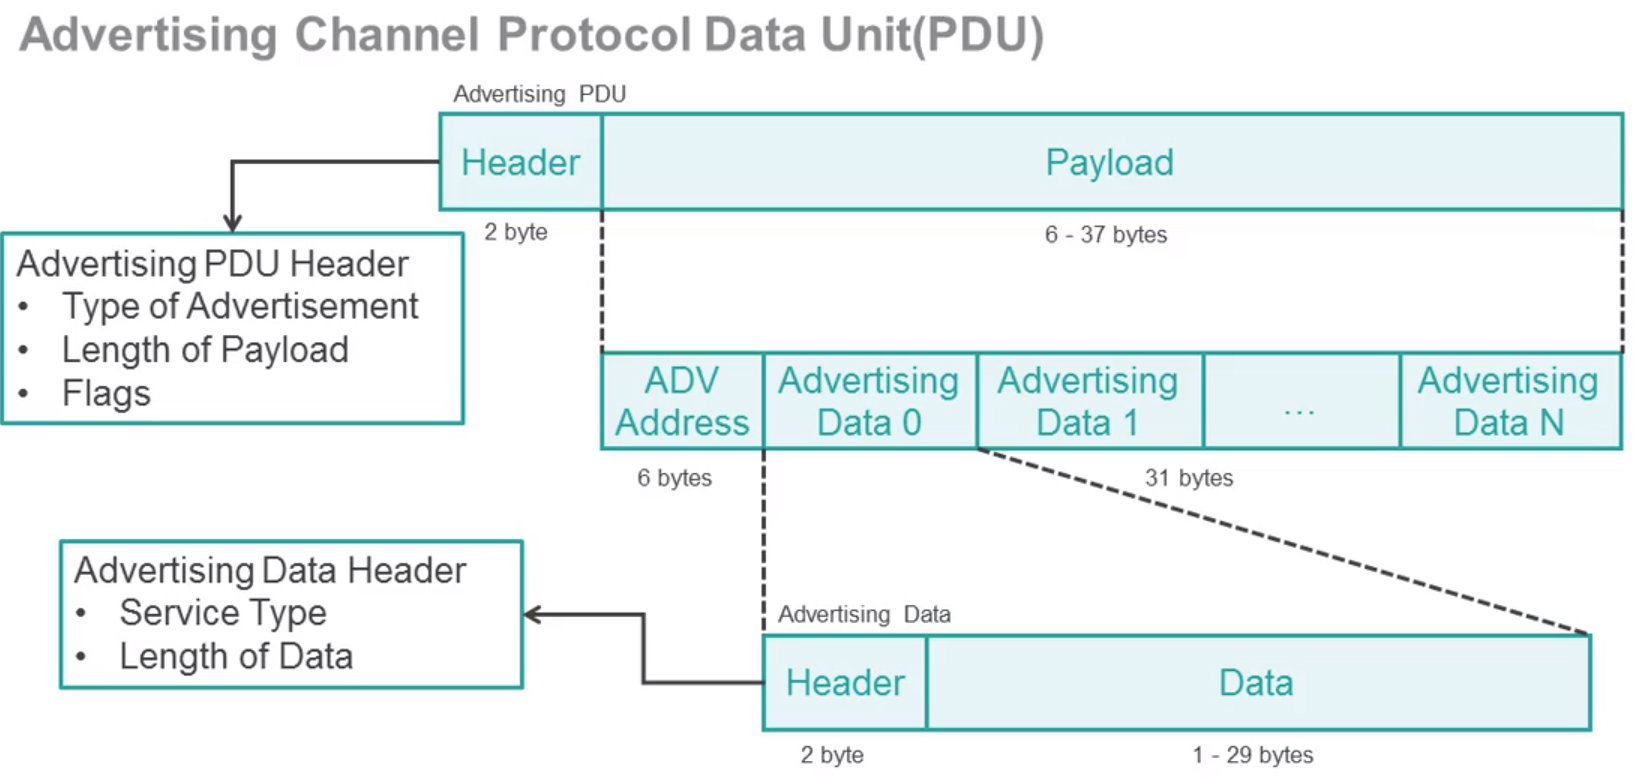
\includegraphics[width=1.0\textwidth]{Figures/Protocols/Bluetooth/ble_adv_packet_content.PNG}
    \caption{Contenu d'un paquet de type \textit{advertisement}}
    \label{fig-ble_adv_packet_content}
\end{figure}

Le contenu d'un \textit{advertisement} est illustré par la \cref{fig-ble_adv_packet_content}. La taille complète d'un \textit{advertisement} ne peut pas dépasser 39 bytes en Bluetooth 4.2. Les deux premiers bytes sont là pour renseigner les dispositifs qui scannent sur les différents paramètres et configurations offerts par le périphérique. Parmi ces informations, il est possible de savoir si le dispositif est connectable, si celui-ci utilise une adresse fixe ou variable, etc. Il indique également s’il est possible de demander au périphérique des informations supplémentaires en effectuant un \textit{Scan Request}, afin de récupérer un nouvel \textit{advertisement} contenant un \textit{Scan Response}. Pour information, le site Internet suivant offre une description très détaillée de chacun des champs et de la valeur qui peut lui être assignée : 
\begin{center}
    \small{\url{http://j2abro.blogspot.ch/2014/06/understanding-bluetooth-advertising.html}}
\end{center}

A la suite de l'entête, se trouve l'adresse MAC du périphérique (fixe ou aléatoire). S'ensuivent différents paquets de données qui sont tous accompagnés d'une nouvelle entête. C'est avec ces derniers qu'il est possible d'implémenter des \textit{beacons} (cf. \cref{sec-protocols_BLE_beacons}).\\

L'intervalle entre les \textit{advertisements} est configurable par le programmeur. Cet intervalle est normalisé et peut varier de 20\,ms à 10.24\,s avec des pas de 0.625\,ms \cite{Lesson3I56:online}. Plus cet intervalle est court, plus la centrale aura de chances de détecter le périphérique. Cependant, cette vitesse se fait au détriment de la consommation énergétique qui sera donc plus importante. L'intervalle inclut un facteur aléatoire dans le temps afin d'éviter les chances de collisions, par exemple, lorsque deux dispositifs avec le même intervalle commencent à émettre des \textit{advertisements} en même temps.

\subsection{Machine des états de la connexion}

\begin{figure}[ht!]
    \centering
    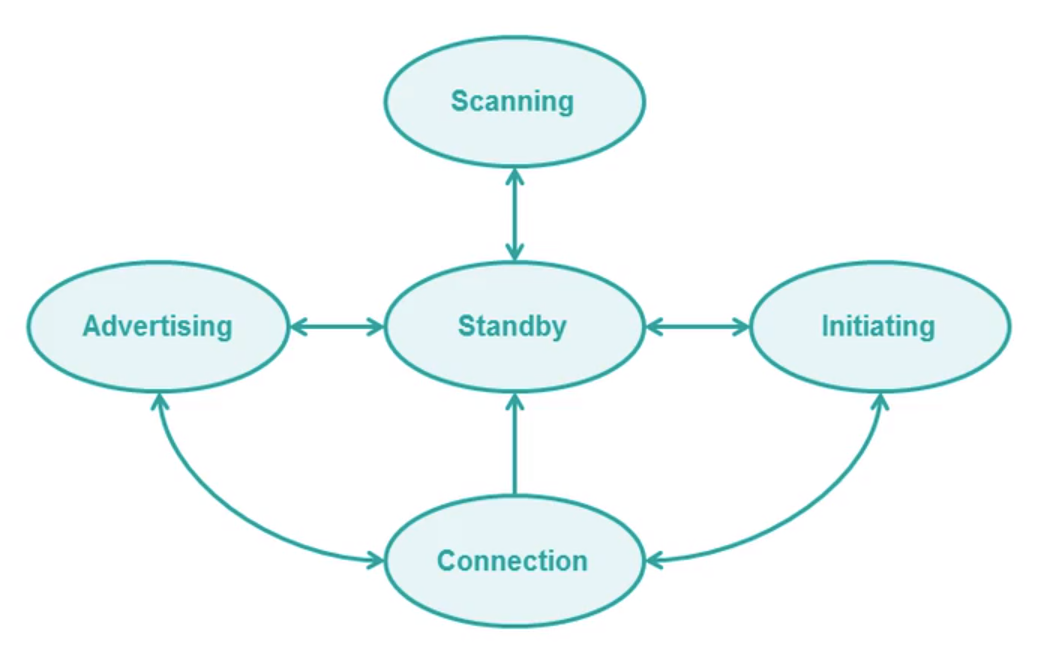
\includegraphics[width=0.8\textwidth]{Figures/Protocols/Bluetooth/state_machine_5_states.PNG}
    \caption{Les 5 états possibles pour un dispositif Bluetooth Low Energy}
    \label{fig-state_machine_5_states}
\end{figure}


Il existe 5 états possibles pour un appareil avec du Bluetooth Low Energy. Ces 5 états sont illustrés sur la \cref{fig-state_machine_5_states}, de même que les liaisons possibles entre ceux-ci. L'explication de ces états est la suivante : 

\begin{enumerate}
    \item \texttt{\textit{Standby}} : état par défaut. C'est dans ce mode que les dispositifs attendent qu'une nouvelle action leur soit demandée. C'est l'état où ils consomment également le moins d'énergie.
    \item \texttt{\textit{Advertising}} : état où le périphérique envoie des \textit{advertisements}, afin de notifier s'il est connectable ou simplement lorsqu'un dispositif souhaite envoyer des données (par exemple des \textit{beacons}).
    \item \texttt{\textit{Scanning}} : état où la centrale scanne ses environs afin de rechercher le dispositif auquel elle souhaite se connecter. Ce mode vise également la situation où la centrale est simplement intéressée par les paquets d'\textit{advertisements} qui transitent, sans forcément vouloir établir une connexion.
    \item \texttt{\textit{Initiating}} : état où la centrale décide de se connecter avec un périphérique. Elle tente de l'atteindre afin d'effectuer une procédure de connexion.
    \item \texttt{\textit{Connection}} : état où les deux périphériques ont acceptés la connexion et peuvent maintenant commencer à s'échanger des données.
\end{enumerate}

\begin{figure}[ht!]
    \centering
    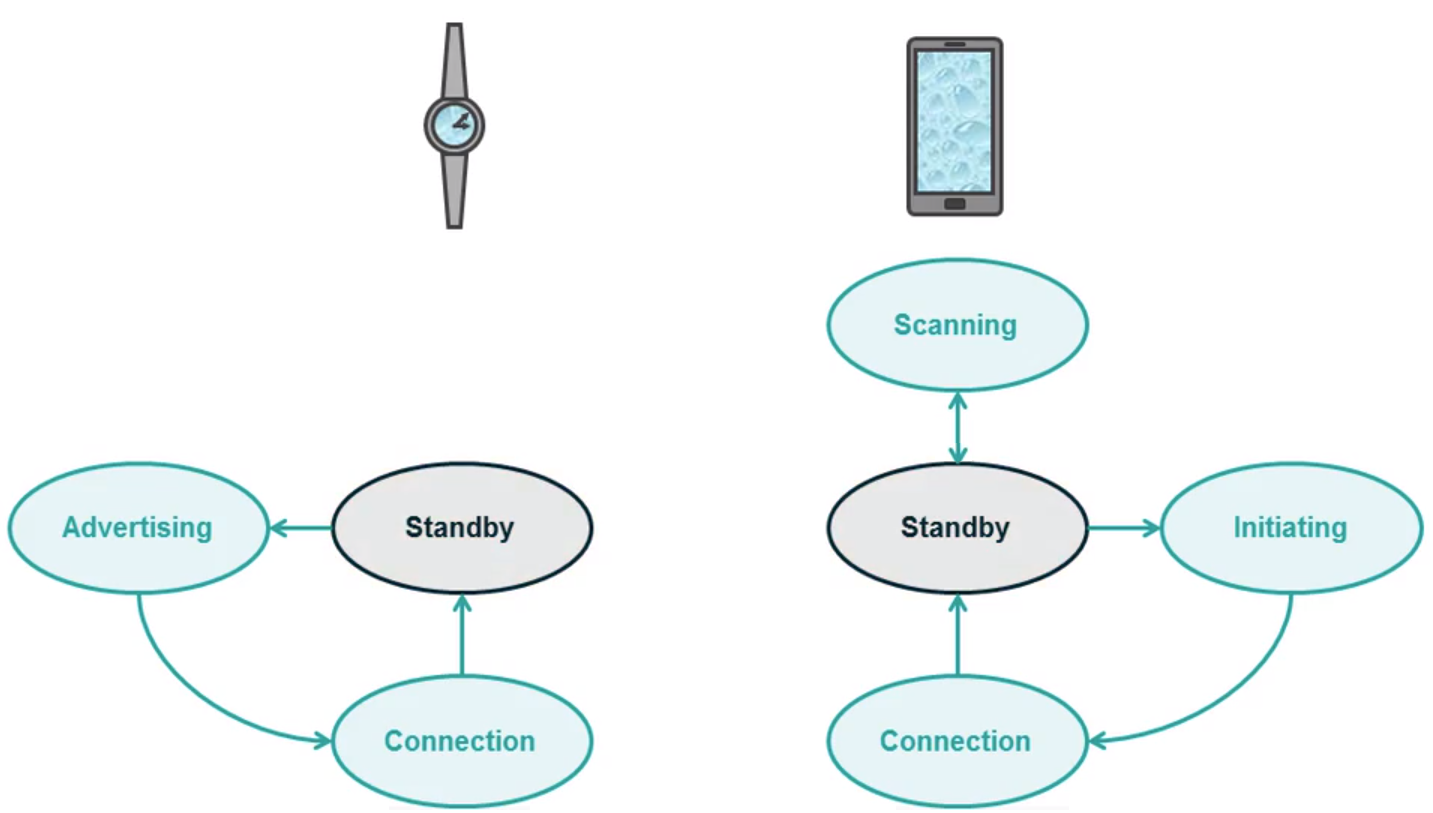
\includegraphics[width=0.8\textwidth]{Figures/Protocols/Bluetooth/states_while_connecting.PNG}
    \caption{Étapes lors de la connexion Bluetooth entre une centrale et un périphérique}
    \label{fig-states_while_connecting}
\end{figure}

Ces 5 états ne sont pas utilisés en parallèle. Un périphérique et une centrale n'en utilisent qu'un nombre limité. La \cref{fig-states_while_connecting} illustre la connexion d'un smartphone en mode central à une montre connectée en tant que périphérique. Voici la séquence de connexion de ces deux dispositifs : 

\begin{enumerate}
    \item Prenons l'exemple où les deux dispositifs commencent en mode \texttt{\textit{Standby}}.
    \item Le périphérique se met en mode \texttt{\textit{Advertising}} lorsqu'il est prêt à être connecté. En parallèle, le smartphone (centrale) se met en mode \texttt{\textit{Scanning}} pour détecter la présence du périphérique périodiquement. 
    \item Lorsque le scanne est fini, la centrale repasse en \texttt{\textit{Standby}}. Si dans ce mode celle-ci détecte la présence de son périphérique via les données reçues de l'état \texttt{\textit{Scanning}}, celle-ci entre en mode \texttt{\textit{Initiating}} afin d'initier une procédure de connexion avec le périphérique.
    \item Si le périphérique accepte la connexion provenant de la centrale, les deux passent alors dans l'état \texttt{\textit{Connection}}. Si la connexion échoue, les deux dispositifs repassent en \texttt{\textit{Standby}}. Le périphérique peut se remettre à générer des \textit{advertisements} s'il le souhaite.
\end{enumerate}


\subsection{Architecture d'une \textit{stack} Bluetooth}

\begin{figure}[ht!]
    \centering
    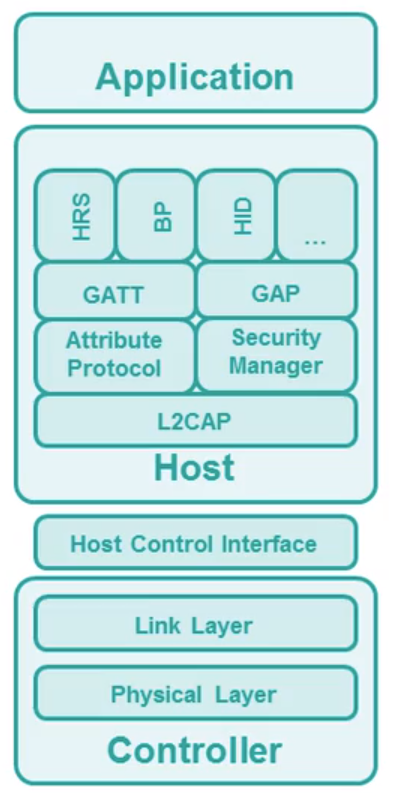
\includegraphics[width=0.3\textwidth]{Figures/Protocols/Bluetooth/ble_full_stack_explained.PNG}
    \caption{Architecture complète de la stack BLE}
    \label{fig-ble_full_stack_explained}
\end{figure}

L'architecture Bluetooth se subdivise en trois dénominations principales, illustrées à la \cref{fig-ble_full_stack_explained}. Ces trois subdivisions se nomment \texttt{Controller}, \texttt{Host} et \texttt{Application}. Entre le \texttt{Controller} et l'\texttt{Host}, il existe un quatrième élément d'interfaçage nommé \textit{Host Control Interface}. Le but de cette sous-section est d'explorer les différents composants de chacune de ces dénominations, afin d'avoir une vue plus complète du protocole Bluetooth Low Energy. Une partie de ces explications proviennent de la vidéo nommée \textit{Lesson 3: Introduction to Bluetooth Low Energy}\footnote{\url{https://www.nxp.com/video/lesson-3-introduction-to-bluetooth-low-energy:LESSON-3-KW41Z-WIRELESS-LAB}} par NXP. 

Dans un OS, ces trois tâches consistent souvent en trois processus bien distincts qui communiquent entre elles avec des interfaces tenant compte des problèmes liés à la concurrence. Il est important de comprendre comment ces trois entités fonctionnent lorsque l'on programme sur un dispositif aussi bas niveau qu'un microcontrôleur. 


\subsubsection{\textit{Controller}}

Le contrôleur est la brique la plus basse du Bluetooth et a pour but de gérer l'interface RF avec les différentes spécificités liées à celle-ci. Elle est dépendante de l'implémentation matérielle du dispositif. Cette interface est différente pour chaque contrôleur utilisé, mais implémente des concepts similaires.

\subsubsubsection{\textit{Physical Layer}}

La couche physique s'occupe de toute la gestion des différents canaux présentés précédemment sur la \cref{fig-ble_channels_vs_802}. Cette couche effectue les décalages en fréquences (\textit{Frequency Hopping Spread Spectrum}), mais ce n'est pas elle qui choisit les \textit{timings} des sauts de fréquences. Son rôle est uniquement de générer la modulation demandée par la couche supérieure, avec les paramètres qui lui sont appliqués.

\subsubsubsection{\textit{Link Layer}}

La couche \texttt{Link Layer} se charge de la gestion des connexions ainsi que de la qualité de celles-ci. Cette couche communique avec la \texttt{Physical Layer} lorsque le \textit{Frequency Hopping Spread Spectrum} doit être adapté en raison d'une saturation du réseau. Cette couche gère également tous les aspects des connexions Bluetooth Low Energy.


\subsubsection{\textit{Host Control Interface}}

Le \texttt{Host Control Interface}, souvent abrégé par \textit{HCI}, est une interface standardisée entre l'Host et le Controller. Cette interface implémente les mêmes concepts, quelleque soit la plateforme. L'avantage de cd type d'interface est de gagner du temps lorsque l'on change de contrôleur RF. Ainsi, seule la brique inférieure doit être modifiée sans influencer celles du dessus. L'interface HCI est également présente dans le Bluetooth \textit{standard}. La base est similaire (entre les deux), mais les \textit{advertisements} et les scans nécessitent de nouvelles commandes. \\

Dans certaines implémentations, le contrôleur est un périphérique externe au microcontrôleur et est connecté à celui-ci à l'aide d'une interface série (UART, SPI, etc.). Aussi, on retrouve le HCI dans ce type d'utilisations, bien que celle-ci soit du côté périphérique et convertisse ensuite les données en série en un format standardisé HCI.

\subsubsection{\textit{Host}}


L'\textit{Host} est l'élément le plus complexe du Bluetooth. Le but de cette section n'est pas d'explorer toutes les spécificités de cet élément, mais de comprendre ses rôles et ses composants principaux.



\subsubsubsection{\textit{L2CAP}}

L2CAP signifie \texttt{Logical link control and adaptation protocol}. Il a les fonctions suivantes : 
\begin{enumerate}
    \item Transporter les données pour les couches de niveau supérieures, avec la gestion du \textit{multiplexing} sur un même lien de données;
    \item Segmenter et réassembler les paquets de données;
    \item Concentrer les données provenant de plusieurs flux en une seule interface;
    \item Gérer la \textit{Quality of Service} pour les couches supérieures. Il s'occupe de la gestion des erreurs et retransmet des données si celles-ci échouent.
\end{enumerate}


\subsubsubsection{\textit{GAP}}
\label{sec-protocols_BLE_GAP}

GAP signifie \texttt{Generic Access Profile}. Il s'agit d'un service Bluetooth Low Energy qui vise à configurer l'accessibilité du périphérique. On trouve les informations suivantes dans ce service : 
\begin{enumerate}
    \item le périphérique peut-t-il être découvert et comment le découvrir;
    \item le périphérique est-il connectable et quelles sont les configurations nécessaires pour mettre en place cette connexion si elle est acceptée.
    \item le périphérique est-il \textit{bondable} (cet aspect sera exploré plus en détail avec la thématique de la sécurité Bluetooth Low Energy de la \cref{sec-security_ble}). 
    \item Une fois le \textit{bond} effectué, le GAP s'occupe de la gestion des clés de sécurité et de l'autorisation des centrales qui peuvent se connecter au périphérique.
\end{enumerate}

Le service GAP définit également les rôles implémentés par le dispositif. Les deux rôles "centrale" et "périphérique" ont été présentés précédemment, mais il existe deux \textit{sous-rôles} : 
 
\begin{enumerate}
    \item \texttt{Broadcaster} : principe appliqué par les dispositifs de type \textit{beacons} (cf. \cref{sec-protocols_BLE_beacons}), c'est un périphérique qui émet des \textit{advertisements,} mais qui n'est jamais connectable.
    \item \texttt{Observer} : scanneur qui scrute en permanence le réseau Bluetooth Low Energy, mais qui n'initie pas de connexion avec un périphérique.
\end{enumerate}

\subsubsubsection{\textit{Security Manager}}
\label{sec-protocols_BLE_security_manager}

Le \texttt{Security Manager} porte, comme son nom l'indique, sur la gestion de tout l'aspect sécurité du périphérique. Il génère les clés lors des différentes connexions. Les clés temporaires sont stockées pour la session active, tandis que des \textit{Long Term Key} (LTK) sont utilisées pour les périphériques \textit{bonded} (cf. \cref{sec-security_ble} pour plus de détails). Ce bloc s'occupe également de chiffrer les données lorsque le type de sécurité appliqué le demande.


\subsubsubsection{\textit{ATT}}

ATT signifie \texttt{Attribute Protocol}. Ce bloc crée les deux interfaces Serveur et Client (cf. \cref{sec-protocol_ble_roles}). Les éléments effectuant la mise à disposition de ces données sont appelés \textit{Attributes} et présentent les caractéristiques suivantes : 
\begin{itemize}
    \item \texttt{Attribute Type} : Un attribut est défini par un identifiant unique. Celui-ci est un UUID\footnote{\url{https://en.wikipedia.org/wiki/Universally_unique_identifier}} sur 128-bit. Cet identifiant peut être raccourci à 16 bits, lorsqu'il s'agit d'identifiants standardisés Bluetooth.
    \item \texttt{Attribute Handle} : définit où l'attribut est sauvegardé sur le serveur.
    \item \texttt{Attribute Value} : comme son nom l'indique, cette caractéristique définit la valeur de l'attribut. La taille maximale assignable à celui-ci est de 512 bytes.
    \item \texttt{Attribute Permissions} : Les permissions définissent les différentes opérations pouvant être effectuées sur l'attribut. Par exemple, \textit{Read}, \textit{Write} ou \textit{Read/Write} simultanément.
\end{itemize}

\begin{figure}[ht!]
\centering
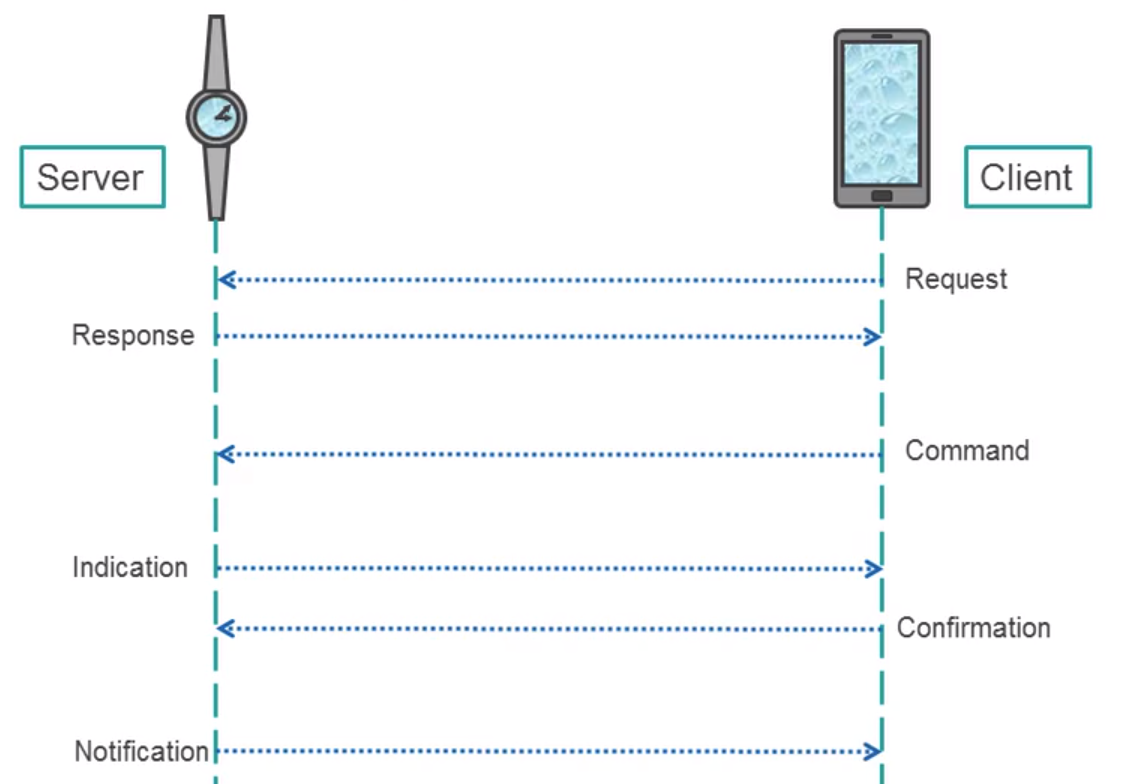
\includegraphics[width=0.8\textwidth]{Figures/Protocols/Bluetooth/client_server_4_operations.png}
\caption{Opérations possibles entre un serveur et un client Bluetooth Low Energy}
\label{fig-client_server_4_operations}
\end{figure}


Une fois connecté, l'accès à un attribut entre un serveur et un client peut s'effectuer à l'aide de quatre opérations. Ces opérations, décrites sur la \cref{fig-client_server_4_operations}, sont les suivantes :
\begin{enumerate}
    \item \texttt{Request/Response} : Lorsque le client souhaite uniquement \underline{lire} un attribut depuis le serveur, il effectue une opération de type \textit{request}. Le serveur lui répond ensuite avec une \textit{response}. 
    \item \texttt{Command} : Lorsque le client souhaite \underline{écrire} un attribut, il effectue une opération de type \textit{command}. Il existe une variante de la commande où il est possible de rajouter une confirmation lors de l'écriture.
    \item \texttt{Indication} : Lorsque le serveur a une nouvelle donnée disponible sur l'attribut, il peut l'envoyer au client sous forme d'\texttt{indication}. Si le client récupère correctement cette donnée, un accusé de réception est envoyé \underline{avec une confirmation} au serveur.
    \item \texttt{Notification} : Lorsque le serveur a une nouvelle donnée disponible sur l'attribut, il peut l'envoyer au client sous forme de notification. Cependant, contrairement à l'indication, la réception de donnée par le client \underline{n'est pas confirmée}. Cela permet ainsi d'économiser des échanges et d'augmenter le débit ou de réduire la consommation. 
\end{enumerate}

\subsubsubsection{\textit{GATT}}

GATT signifie \texttt{Generic Attribute Profile}. C'est une couche au-dessus de l’ATT qui a pour but de hiérarchiser les différents groupes d'attributs en un concept nommé \texttt{\textbf{Services Bluetooth Low Energy}}. 

Le GATT gère également la découverte de ces divers services en répondant aux requêtes de type \texttt{Discovery Services} d'un client. Le format pour la découverte est doté de diverses règles qui sont appliquées par le GATT.


\subsubsubsection{\textit{Profils et services}}
\label{sec-protocols_BLE_services}

Sur la \cref{fig-ble_full_stack_explained} on peut remarquer la présence de plusieurs blocs au-dessus du GATT. Il s'agit là de services GATT standardisés. Trois services sont listés : 
 \begin{itemize}
     \item \texttt{HRS} : signifie \textit{Heart Rate Service}
     \item \texttt{BP} : signifie \textit{Blood Pressure Service}
     \item \texttt{HID} : signifie \textit{Human Interface Device Service}, lequel offre ainsi la possibilité de connecter des périphériques à l'aide du Bluetooth Low Energy (ex. souris sans fil)
 \end{itemize}


Ces services sont intégrés dans des \textbf{profils} standardisés par le protocole Bluetooth : 
\begin{center}
    \url{https://www.bluetooth.com/specifications/gatt}
\end{center}

Le but de ces profils standardisés est d'augmenter l'interopérabilité des différents appareils avec les interfaces de données standards. Par exemple, dans le cas d'un HRS, l'interface de capture du système cardiaque est standard, ce qui permet à n'importe quel développeur de faire une application générique pour tous les capteurs cardiaques du marché. \\

Si un développeur souhaite créer son propre profil, il doit se plier à certaines restrictions quelques restrictions. Les UUIDs des attributs ne peuvent pas utiliser l'UUID attribué aux services Bluetooth standardisés, à savoir la valeur \path{0000XXXX-0000-1000-8000-00805f9b34fb}. Les \texttt{XXXX} représentent le UUID 16 bits pouvant être utilisés au lieu des 128 bits, lorsque les services standards sont accédés. La liste complète de ces services, ainsi que leur UUID 16bit, est disponible à l'adresse suivante : 
\begin{center}
    \url{https://www.bluetooth.com/specifications/gatt/services}
\end{center}



\begin{table}[ht!]
\centering
\caption{Paramètres d'un \textit{Client Characteristic Configuration Descriptor}}
\label{tab-cccd_parameters}
\begin{tabular}{|l|l|l|l|}
\hline
\multicolumn{4}{|l|}{\cellcolor[HTML]{BBDAFF}{\color[HTML]{333333} \textbf{Bit Field Client Characteristic Configuration (CCCD)}}} \\ \hline
                                      &                                       & \multicolumn{2}{l|}{\textbf{Definition}}           \\ \cline{3-4} 
\multirow{-2}{*}{\textbf{Bit}}        & \multirow{-2}{*}{\textbf{Size}}       & \textbf{Key}       & \textbf{Value}                \\ \hline
                                      &                                       & 0                  & Notifications disabled        \\ \cline{3-4} 
\multirow{-2}{*}{0}                   & \multirow{-2}{*}{1}                   & 1                  & Notifications enabled         \\ \hline
                                      &                                       & 0                  & Indications disabled          \\ \cline{3-4} 
\multirow{-2}{*}{1}                   & \multirow{-2}{*}{1}                   & 1                  & Indications enabled           \\ \hline
                                      &                                       & 0                  & Reserved for future use       \\ \cline{3-4} 
\multirow{-2}{*}{2 to 15}             & \multirow{-2}{*}{14}                  & 1                  & Reserved for future use       \\ \hline
\end{tabular}
\end{table}


La couche ATT indique que tout élément avec un UUID est un attribut. Au niveau GATT, on utilise toutefois des définitions différentes pour chaque élément. Un \textbf{service} ne produit pas de données, son unique rôle étant de définir une encapsulation pour des \textbf{caractéristiques}. Ce sont les caractéristiques qui contiennent toutes les données des capteurs. Une caractéristique peut ensuite être accompagnée de plusieurs \textbf{descripteurs}\footnote{\url{https://www.bluetooth.com/specifications/gatt/descriptors}}. Les descripteurs ont pour rôle de configurer ou simplement d'informer une caractéristique. Le descripteur le plus connu et utilisé est le \texttt{Client Characteristic Configuration Descriptor} (CCCD). Si une caractéristique est autorisée à envoyer ses données en tant que notifications ou indications, l'utilisateur doit configurer ce descripteur pour activer ces fonctionnalités. Les paramètres possibles de ce descripteur sont visibles sur la \cref{tab-cccd_parameters}. 


\begin{figure}[ht!]
\centering
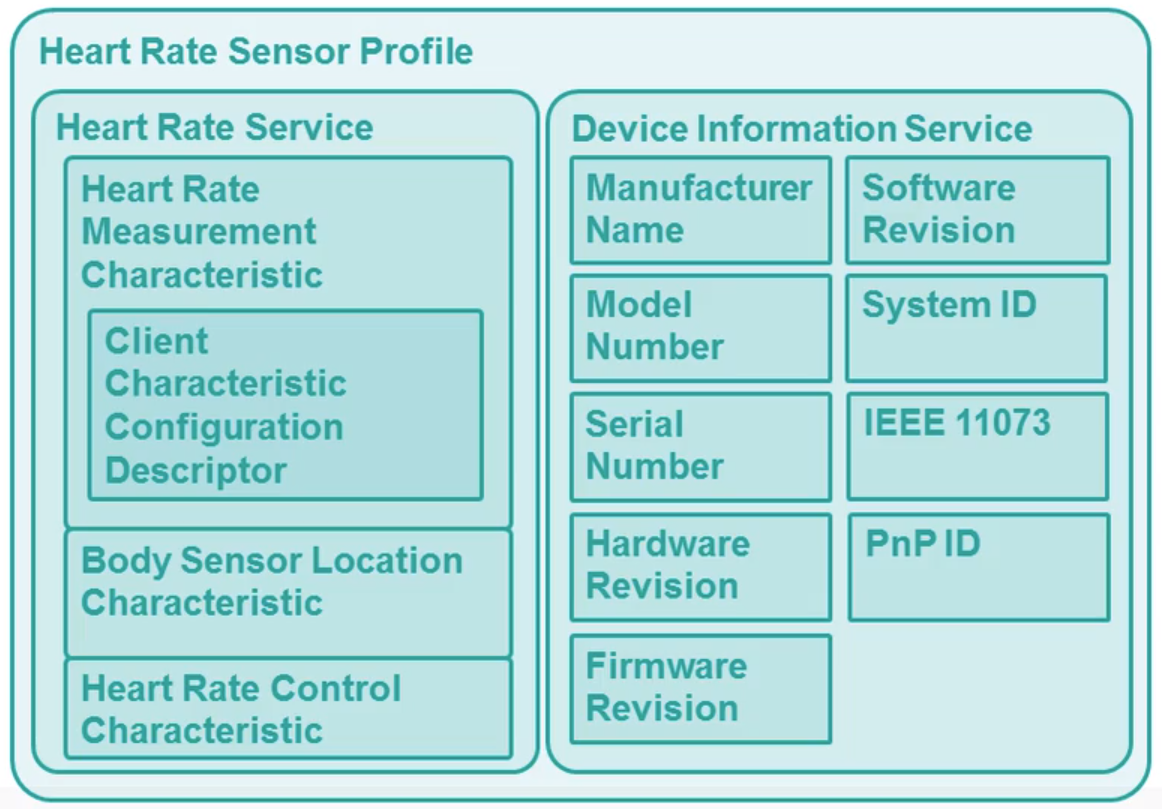
\includegraphics[width=0.6\textwidth]{Figures/Protocols/Bluetooth/heart_rate_sensor_profile.png}
\caption{Profil \textit{Heart Rate Sensor} standardisé}
\label{fig-heart_rate_sensor_profile}
\end{figure}

Lorsqu'un développeur crée un profil, il doit parfaitement comprendre ses couches intérieures afin que son implémentation soit correcte. Si on reprend l'exemple du \textit{HRS}, dont les éléments sont visibles sur la \cref{fig-heart_rate_sensor_profile}, on y voit le contenu complet qui doit être implémenté pour qu'un dispositif soit compatible avec ce profil. On a tout d'abord deux services, le principal étant celui de la mesure cardiaque. Le deuxième est le \texttt{Device Information Service}, qui comme son nom l'indique, fournit des informations sur le périphérique. Il y a ensuite la présence de trois caractéristiques : la \texttt{Heart Rate Control} permet de configurer le temps entre chaque nouvelle acquisition de valeur; La \texttt{Body Sensor Location}, qui informe sur l'emplacement du corps où le périphérique est situé; la \texttt{Heart Rase Measurement}, caractéristique la plus importante qui fournit la fréquence capturée par le capteur cardiaque. Cette caractéristique est disponible en tant que notification ou indication, puisqu'elle est également constituée d'un CCCD. Si deux profils demandent l'implémentation du même serveur, par exemple le \texttt{Device Information Service}, celui-ci n'a besoin d'être implémenté qu'une seule fois.


\subsubsection{\textit{Application}}

L'application est là où toutes les données des services sont acquisitionnées. Les communications avec les capteurs sont effectuées à ce niveau, puis une fois les données récupérées, elles sont inscrites dans les attributs ATT correspondants, à travers la base de données GATT.


\subsection{Beacons}
\label{sec-protocols_BLE_beacons}

En principe, il est possible de savoir combien de dispositifs sont présents simplement en effectuant un scan. Si l'utilisateur a son Bluetooth activé, le système va périodiquement scanner ses environs et communiquer son adresse MAC lors des réponses aux \textit{Scan Requests}. Cependant, depuis la norme 4.0 du Bluetooth Low Energy (améliorés avec la norme 4.2\cite{Bluetoot24:online}), les périphériques doivent supporter le principe de Low Energy (LE) Privacy\cite{Bluetoot24:online}. Il ne doit pas forcément être activé par défaut, mais cette option doit être implémentée sur tous les contrôleurs Bluetooth 4.2. Ce mode a pour but de modifier périodiquement l'adresse MAC du périphérique lorsque celui-ci envoi des \textit{advertisements}. Cela a pour effet d'empêcher la traque de personnes à leur insu, au moyen d'une simple borne qui scan tous les périphériques à proximité. Le microcontrôleur KW41Z supporte ce mode, comme tous les smartphones iOS ou Android. Le but étant de scanner le nombre de personnes autour d'une borne, il faut pouvoir détecter ces personnes par un moyen sûr. Les systèmes d'exploitation des smartphones (iOS et Android) ont activé par défaut le mode privacy sans possibilité de le désactiver pour les programmeurs. La fréquence du changement d'adresse MAC enduite par le LE Privacy est de l'ordre de 3min sur un smartphone, mais celle-ci varie selon les modèles de \textit{smartphones} et n'est pas configurable par le développeur. \\

Pour pallier à cette limitation, le principe de \textit{beacons} s'est très vite répandu. Il s'agit alors de modifier le contenu d'un paquet \textit{advertisement} afin d'y placer un \textit{payload} personnalisable. La transmission d'un \textit{beacon} est unidirectionnelle. Le périphérique qui scanne les \textit{beacons} ne peut pas directement interagir avec eux. Normalement, le scanner a uniquement besoin de connaitre les périphériques qui l'entoure, ainsi que la distance qui les sépare (calculable avec la puissance du signal RSSI). Les \textit{beacons} ont tous une taille de paquet maximale de 31 bytes (cf. \cref{sec-protocol_ble_adv}), dont trois bytes réservés au champ \textit{Advertisement Flag} (Adv Flag) obligatoire.

Il existe trois spécifications de \textit{beacons} principalement utilisées \cite{Understa87:online} : 

\begin{enumerate}

\begin{figure}[ht!]
\centering
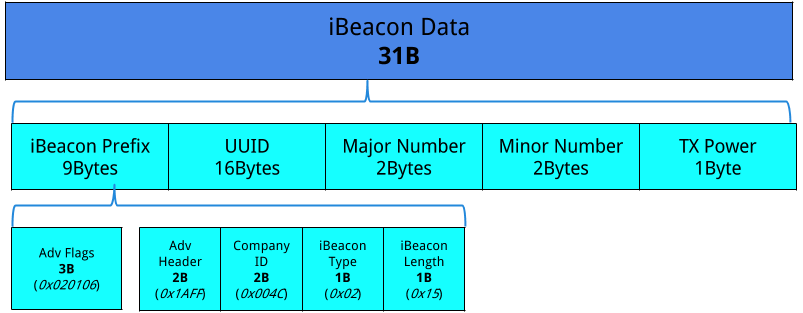
\includegraphics[width=0.8\textwidth]{Figures/Protocols/Bluetooth/ibeacon-spec-exploded-view.png}
\caption{Spécification des paquets iBeacons}
\label{fig-ibeacon-spec-exploded-view}
\end{figure}

    \item iBeacons : spécification de protocole développé par Apple\footnote{\url{https://developer.apple.com/ibeacon/}}. Le contenu du paquet BLE est affiché sur la \cref{fig-ibeacon-spec-exploded-view}. Le paquet contient un entête constitué d'un \textit{Company ID}, lequel doit être délivré par Apple pour chaque fabricant de \textit{beacons} afin que celui-ci soit conforme à la spécification. On a ensuite un UUID, unique pour chaque \textit{beacon}, \textit{Major} qui identifie un sous-réseau de plusieurs \textit{beacons} et un \textit{Minor} qui identifie un \textit{beacon} précis. L'utilisateur peut ensuite utiliser ces trois identifiants pour récupérer les informations sur le \textit{beacon} dans une base de données. En fin du paquet, il y a la puissance d'émission en dBm à 1m afin d'estimer la distance en fonction du RSSI mesuré par le scanneur. Le paquet fait au total 31 bytes, mais uniquement 20 bytes (UUID, \textit{Major} et \textit{Minor}) sont configurables par l'utilisateur, le reste étant fixé par Apple ou le fabricant certifié du \textit{beacon}.
    

\begin{figure}[ht!]
\centering
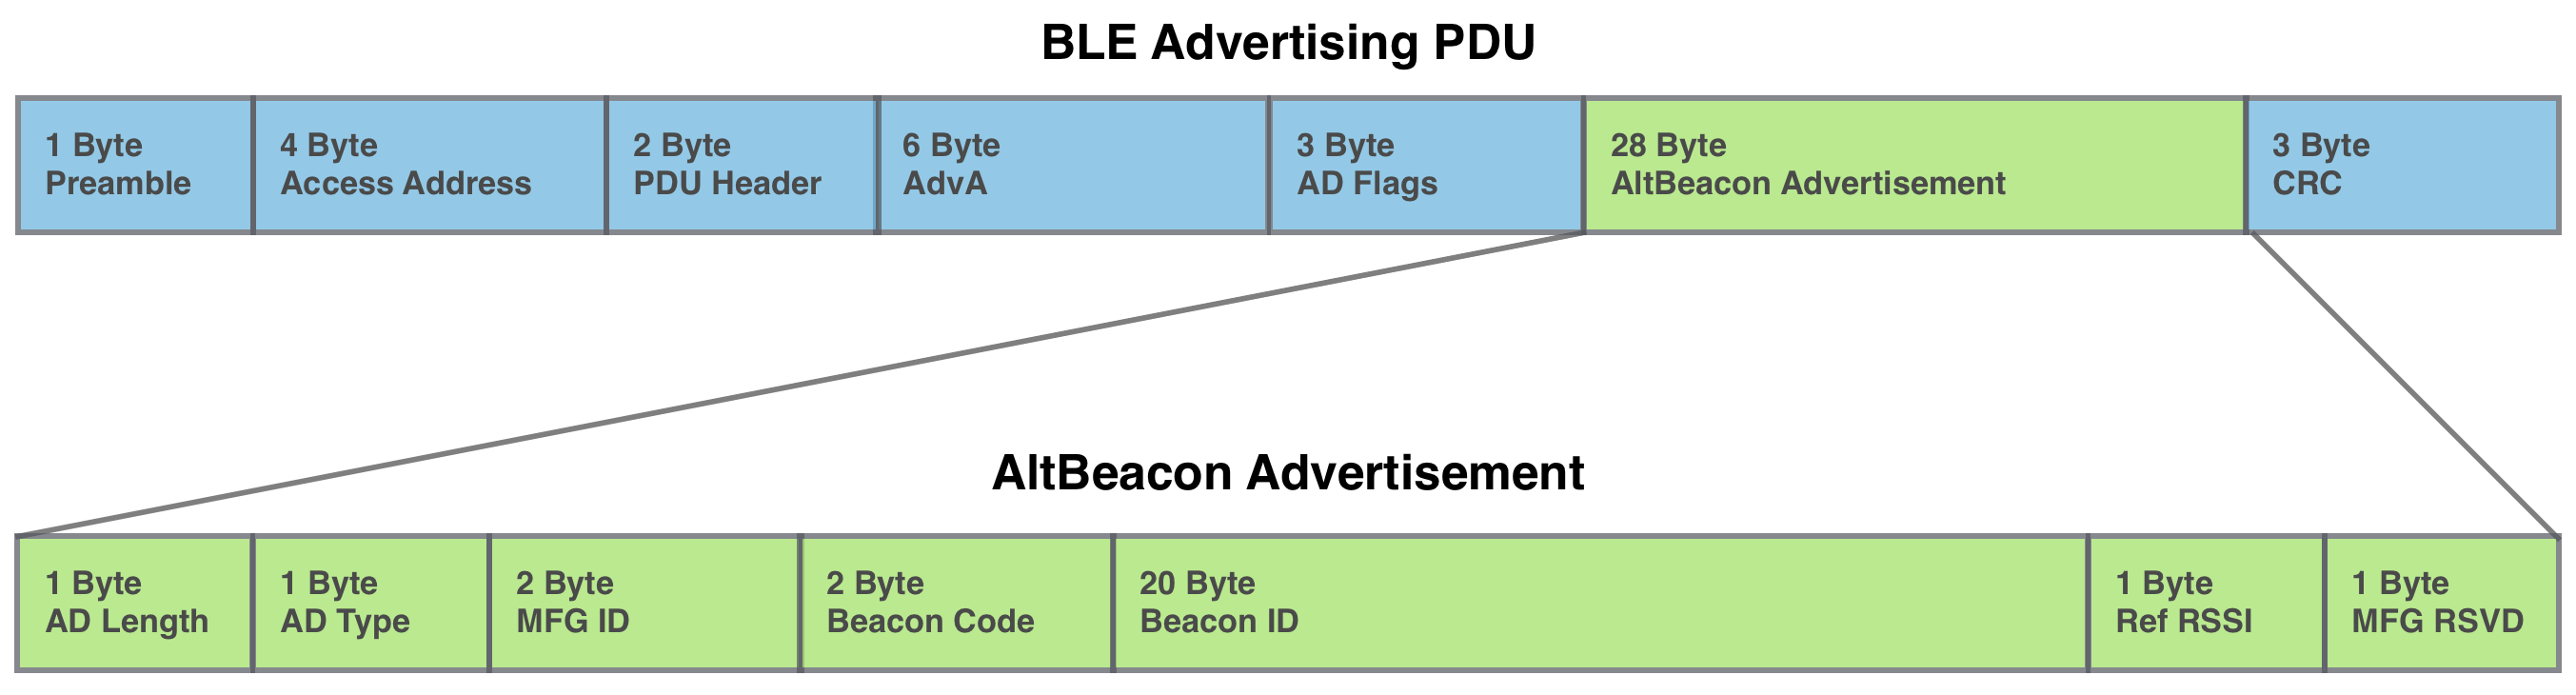
\includegraphics[width=1.0\textwidth]{Figures/Protocols/Bluetooth/altbeacon-spec-exploded-view.png}
\caption{Spécification des paquets AltBeacon}
\label{fig-altbeacon-spec-exploded-view}
\end{figure}

    \item AltBeacon : spécification de protocole développé par Radius Networks \footnote{\url{http://altbeacon.org/}}. Le contenu du paquet BLE est affiché sur la \cref{fig-altbeacon-spec-exploded-view}. Le contenu du champ Beacon ID est identique à l'identifiant utilisé par le iBeacon, c'est-à-dire l'utilisation d'un UUID sur 16 bytes couplé à un \textit{Major} et \textit{Minor} sur deux bytes chacun. L'AltBeacon a 25 bytes modifiables par l'utilisateur, car les champs \textit{Manufacturer ID }(MFG ID), \textit{Beacon Code} et \textit{Manufacturer Reserved Data} (MFG RSVD) sont tous configurables par l'utilisateur. 


\begin{figure}[ht!]
\centering
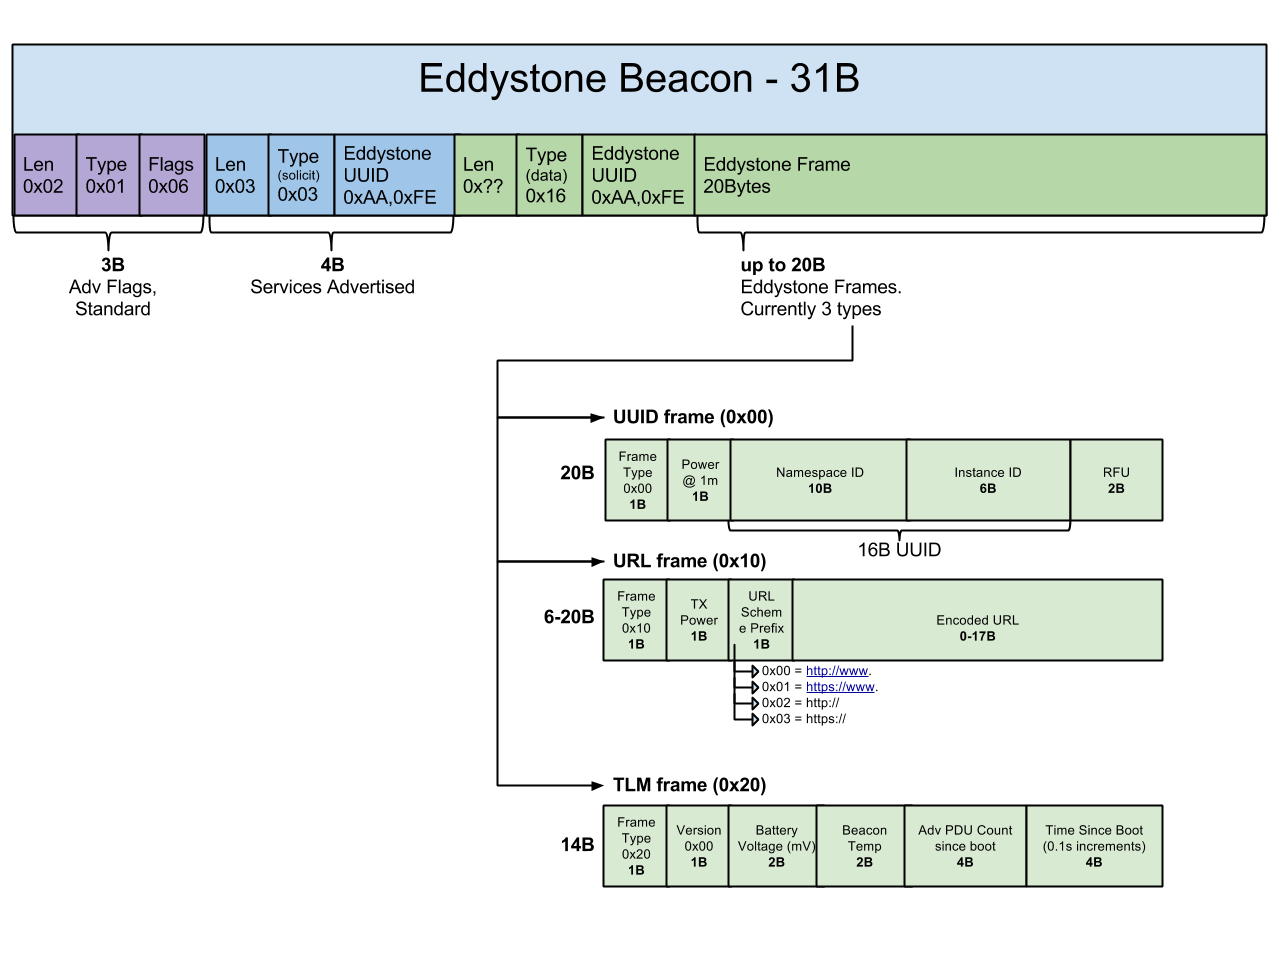
\includegraphics[width=1.0\textwidth]{Figures/Protocols/Bluetooth/eddystone-spec-exploded-view.png}
\caption{Spécification des paquets Eddystone}
\label{fig-eddystone-spec-exploded-view}
\end{figure}
    \item Eddystone : spécification de protocole développé par Google \footnote{\url{https://github.com/google/eddystone}} et initialement appelée URIBeacon. Le contenu du paquet BLE est affiché sur la \cref{fig-eddystone-spec-exploded-view}. Cette spécification a un but différent des deux autres précédemment décrites. Celle-ci fait partie de l'initiative Physical Web\footnote{\url{http://google.github.io/physical-web/}}, qui a pour objectif de faciliter l'interaction avec les objets qui entourent les utilisateurs sans nécessiter une connexion Bluetooth. Il existe trois types de paquets Eddystone :
    \begin{enumerate}
        \item \texttt{UUID} : similaire aux deux technologies précédentes, son but est de diffuser une UUID de 16 bytes découpés en deux champs de 10 et 6 bytes.
        \item \texttt{URL} : Le \textit{beacon} peut diffuser une URL qui peut être lue par un client avec un accès internet. Il peut par exemple diffuser l'URL \url{https://goo.gl/Aq18zF} et chaque client recevant ce paquet pourra visiter le site sur son téléphone. La navigateur Google Chrome sur Android offre ainsi la possibilité de scanner ses environs à la recherche de périphériques proposant des URL Eddystones.
        \item \texttt{TLM} : Offre la possibilité de diffuser des informations télémétriques sur le \textit{beacon}. On peut ainsi connaitre la batterie du périphérique, la température ainsi que le nombre d'\textit{advertisements} envoyés depuis qu'il a démarré. 
    \end{enumerate}
    La spécification UUID est la plus intéressante, mais elle reste plus limitée que le iBeacon ou l'AltBeacon. En effet, elle n'offre que 16 bytes modifiables.
\end{enumerate}



Le but principal de ces \textit{beacons} est d'informer l'utilisateur sur les événements survenant autour de lui, mais ceux-ci peuvent être détournés pour localiser les gens. En effet, si on place des \textit{beacons} fixes, on peut ensuite remonter via Internet la liste des \textit{beacons} à proximité et leurs puissances. Si un grand nombre de \textit{beacons} sont à proximité, il est donc possible de traquer une personne à quelques mètres près. Pour ce faire, une application smartphone qui scan les \textit{beacons} et qui remonte les informations à un serveur est nécessaire. Par contre, conscient de cette invasion de la privacité, les développeurs doivent maintenant demander les droits de localisation sur l'application (même principe pour iOS et Android) afin d'effectuer des scans lorsque le téléphone est en veille.

\FloatBarrier



\subsection{Consommation énergétique}


Le Bluetooth Special Interest Group (SIG) affirme que le BLE consomme entre 1 et 50\,\%, de la consommation du Bluetooth Classic \cite{BLEConsumption:online}. Ce gap oscille selon l'application souhaitée. La \cref{fig-power_consumptions_ble_advertising} illustre la consommation des périphériques en mode \textit{advertising} \cite{BLECONSUMPTIONPUBLICATION}. On constate que les facteurs qui influencent sur la consommation sont: la taille des paquets, l'intervalle entre chaque paquet et la puissance d'émission. Lorsque l'utilisateur le développeur souhaite optimiser la consommation il doit tenir compte de ses trois paramètres. Selon les systèmes utilisés, ces paramètres ne sont pas flexibles. Par exemple, sur Android, le développeur peut uniquement mettre trois modes de fréquences pour le paquet Bluetooth sans jamais pouvoir spécifier un intervalle temporel. Le temps ensuite appliqué varie selon le modèle du périphérique.

\begin{figure}[ht!]
\centering
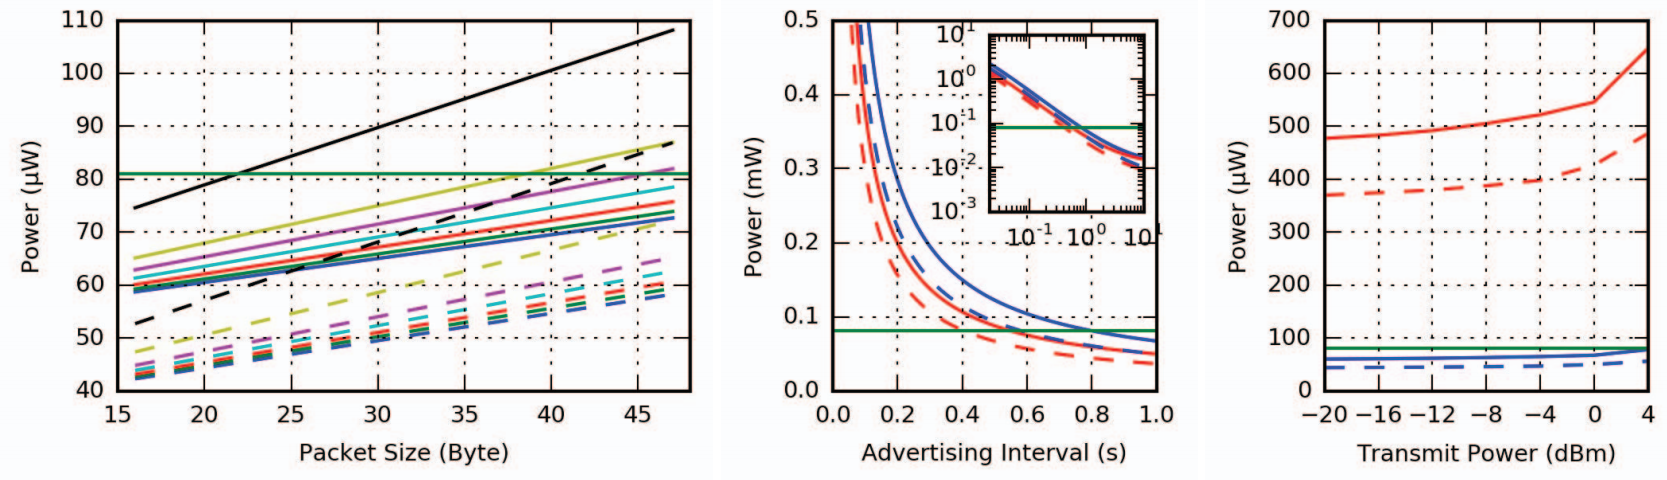
\includegraphics[width=1.0\textwidth]{Figures/Protocols/Bluetooth/power_consumptions.png}
\caption{Consommation des \textit{advertisements} en Bluetooth Low Energy}
\label{fig-power_consumptions_ble_advertising}
\end{figure}



\FloatBarrier



